\documentclass[11pt]{article}
\usepackage[margin=1in]{geometry}
\usepackage{graphicx}
\usepackage{booktabs}
\usepackage{amsmath,amssymb}
\usepackage{microtype}
\usepackage{hyperref}
\usepackage{xcolor}
\usepackage{enumitem}
\usepackage[T1]{fontenc}
\usepackage[utf8]{inputenc}
\usepackage{float}
\usepackage{tcolorbox}
\tcbuselibrary{breakable}
\usepackage{tikz}

\graphicspath{{../results/figures/}}

\definecolor{boxblue}{RGB}{230,238,250}
\definecolor{boxyellow}{RGB}{255,246,220}
\definecolor{boxgreen}{RGB}{230,246,230}
\definecolor{boxred}{RGB}{253,232,232}

\newtcolorbox{jargon}[1]{colback=boxblue,colframe=blue!55!black,
  title={Jargon unpacked: #1},fonttitle=\bfseries,breakable}
\newtcolorbox{whyblock}{colback=boxyellow,colframe=orange!60!black,
  title={Why we do this},fonttitle=\bfseries,breakable}
\newtcolorbox{resultbox}{colback=boxgreen,colframe=green!45!black,
  title={What this number means},fonttitle=\bfseries,breakable}
\newtcolorbox{pitfall}{colback=boxred,colframe=red!60!black,
  title={Pitfall / honest caveat},fonttitle=\bfseries,breakable}

\title{The ``Everything Explained'' Guide\\
\large{A newbie-friendly walkthrough of the Ablation-First\\
Trajectory Analysis of Alveolar Epithelial Robustness Collapse\\
in Lethal COVID-19}}
\author{Systems Biology class project}
\date{\today}

\begin{document}
\maketitle

\begin{abstract}
\noindent This is the long-form, beginner-friendly companion to the paper. It assumes
you have never touched single-cell RNA sequencing, never heard of diffusion
pseudotime, and never dissected a lung. By the end you should be able to tell a
friend, in your own words: (1) what the scientific question is; (2) what every
technical term in the paper means; (3) where the data came from and how it got
onto my computer; (4) every command I ran and what it computed; (5) how to look
at every figure, plot and table and pull the correct conclusion from it;
(6) how the final claim was assembled from those pieces; (7) what I am NOT
claiming and why.

Boxes are colour-coded:
\begin{itemize}
\item Blue boxes unpack technical jargon.
\item Yellow boxes say \emph{why} we do a step (not just what).
\item Green boxes interpret a specific number, plot, or table.
\item Red boxes flag pitfalls, retractions, or limitations I'm being honest about.
\end{itemize}
\end{abstract}

\tableofcontents
\bigskip
\hrule
\bigskip

% =========================================================================
\section{Part 1 --- Start here: the question in plain English}
% =========================================================================

Your lungs are made of about 480 million microscopic air sacs (alveoli).
Their inner wall is a thin sheet of cells --- the alveolar epithelium ---
and this is where oxygen crosses into your blood. In people who died of
severe COVID-19, this sheet is visibly broken: cells are missing, cells are
abnormal, and new-looking cells appear in places they shouldn't.

The specific question of this project is:
\begin{quote}
\textbf{When the alveolar epithelium fails in lethal COVID-19, does it fail in a
\emph{coordinated} way (every sick cell moves toward one damaged state), or does
it fail in a \emph{chaotic} way (cells fan out in many different directions at
once)?}
\end{quote}

These two possibilities are geometrically different and they predict different
things about the data we can measure:

\begin{itemize}
\item If it's \textbf{coordinated}: the COVID cells as a group should sit at a
      clearly different spot from the healthy cells. Their group ``average''
      (centroid) has moved.
\item If it's \textbf{chaotic}: the COVID cells' group average may not move much,
      but the \emph{spread} of COVID cells --- how far each one sits from its
      own group --- should be much larger than in healthy cells.
\end{itemize}

I call the chaotic pattern ``robustness collapse'': the tissue loses its ability
to keep every cell in a tight, healthy identity, so cells drift apart from one
another along many axes of gene expression at once.

\begin{jargon}{what ``robustness'' means here}
In a healthy organ, cells of a given type (e.g.\ every AT2 cell) look very
similar to each other. That uniformity is a sign of a working regulatory
network that pins cells into a shared identity. Stress or damage can weaken
this pinning, so cells drift apart. The \emph{loss of uniformity} itself is
the signature of collapse --- even if no single ``damaged'' state is reached.
\end{jargon}

\begin{whyblock}
This is why I have to measure \emph{two different things} and not just one.
Measuring only the group average (centroid displacement) would miss the chaotic
pattern. Measuring only the spread (dispersion) would miss the coordinated
pattern. So I measure both, on purpose, and I commit to declaring in advance
which outcome supports which hypothesis.
\end{whyblock}

\paragraph{What this project is NOT.}
I am \textbf{not} discovering new biology about COVID-19 lungs.
Melms et al.\ (2021), Delorey et al.\ (2021), and Bharat et al.\ (2020) already
showed alveolar injury, transitional cell accumulation, and donor heterogeneity.
My contribution is \textbf{methodological}:
\begin{enumerate}
\item Pre-register multiple geometric success criteria that would each support
      a different mechanism.
\item Stress-test the conclusions with ten systematic ablations.
\item Audit with an independent 618-donor out-of-cohort replication.
\item Report honestly which signatures survive and which don't.
\end{enumerate}

% =========================================================================
\section{Part 2 --- Biology in plain terms}
% =========================================================================

\subsection{The alveolar epithelium: a two-cell sheet}

Two major epithelial cell types sit on the inner wall of each alveolus:

\begin{description}[style=nextline]
\item[AT1 cells (alveolar type 1)] Very flat, very thin. They cover
$\approx$95\% of the alveolar surface. Their job is \emph{gas exchange}:
oxygen in, carbon dioxide out. They are terminally differentiated (they do
not divide).
\item[AT2 cells (alveolar type 2)] Cube-shaped, smaller surface coverage.
They have two jobs: (i) secrete \emph{surfactant}, a soapy fluid that stops
the alveolus collapsing when you exhale; (ii) serve as local \emph{stem cells}:
when AT1 cells die, AT2 cells divide and transform into new AT1 cells through
a temporary, fragile state called the \emph{transitional} or \emph{DATP}
state (``damage-associated transient progenitor'').
\end{description}

\begin{jargon}{DATP / transitional cell}
A cell that used to be AT2 and is in the process of becoming AT1. It has a
very characteristic gene signature (strong expression of KRT8, CLDN4, SFN;
weaker canonical AT2 markers; partial AT1 markers). In healthy adult lung
these cells are rare. In acute lung injury (including COVID-19 and
pulmonary fibrosis) they accumulate.
\end{jargon}

\subsection{Why COVID-19 hurts this particular sheet}

SARS-CoV-2 enters AT2 cells through the ACE2 receptor. This is bad news because
AT2 cells are simultaneously:
\begin{itemize}
\item The cells making surfactant (so when they fail, alveoli collapse).
\item The local stem cells (so when they fail, AT1 cells can't be replaced).
\end{itemize}
On top of the direct viral damage, the body's inflammatory response chews up
epithelium as collateral damage. In lethal cases, autopsies show \emph{diffuse
alveolar damage}: holes in the AT1 sheet, edema, and abnormal cells caught
mid-transition.

\begin{jargon}{snRNA-seq (single-nucleus RNA sequencing)}
A variant of single-cell RNA sequencing. Instead of isolating whole cells
(which fall apart in frozen post-mortem tissue), you isolate individual
cell \emph{nuclei}. Each nucleus' messenger RNA is barcoded and sequenced,
giving you a counts-per-gene vector per nucleus. People use it for autopsy
and frozen tissue where whole cells cannot be recovered.
Trade-off: you lose a bit of cytoplasmic RNA and gain slightly more nascent
(unspliced) transcript, which shifts what you measure.
\end{jargon}

\subsection{Vocabulary you will meet again}

\begin{description}[style=nextline,leftmargin=0pt]
\item[Gene expression] The amount of messenger RNA produced from a gene in a
      cell at a moment in time. We measure it as a count (UMIs).
\item[Expression vector of a cell] A long list of numbers, one per gene,
      describing how much of each gene that cell was making.
\item[Matrix \texttt{X}] All the expression vectors stacked: rows = cells,
      columns = genes. This is the fundamental data object.
\item[UMI] Unique Molecular Identifier. A short random DNA tag added to each
      RNA molecule before amplification, so we can count distinct molecules
      rather than PCR duplicates.
\item[HVG (Highly Variable Gene)] A gene that differs a lot between cells.
      We keep these for downstream analysis because they carry most of the
      structural signal; the rest are mostly noise.
\item[PCA (Principal Component Analysis)] A way to compress the very long
      expression vector down to (say) 50 numbers that preserve most of the
      variance. Each of the 50 numbers is a ``principal component'' (PC).
\item[UMAP] A non-linear algorithm that takes the 50-number PCA summary and
      places each cell on a 2-D map. Cells near each other on the map had
      similar expression profiles. \emph{It's for seeing, not for measuring.}
\item[Diffusion map / diffusion pseudotime (DPT)] A mathematically principled
      way to build a 1-D ordering of cells that reflects continuous
      transitions along a biological process. If you root it at a ``starting''
      cell and treat cell-cell similarity as a probability of stepping from
      one cell to another, cells that are ``further along the journey'' get
      larger pseudotime values.
\item[Gene program] A hand-curated list of genes that together reflect one
      biological process (e.g.\ the interferon response). We can score each
      cell with one number per program by averaging (roughly) the expression
      of that program's genes.
\item[Batch effect] Systematic differences in the data that come from
      technical stuff (which donor, which day, which chemistry) rather than
      biology.
\item[Batch correction (Harmony)] An algorithm that adjusts the PCA
      coordinates to remove batch-specific shifts while trying to preserve
      real biological structure.
\item[Ablation] In ML/analysis papers, ``ablation'' means systematically
      removing or changing one piece of the pipeline to see if the
      conclusion still holds. If it does, the conclusion is robust. If it
      doesn't, you have learned exactly which pipeline choice was
      load-bearing.
\end{description}

% =========================================================================
\section{Part 3 --- Where the data came from}
% =========================================================================

\subsection{Primary cohort: SCP1219 (Melms 2021)}

This is a publicly released single-nucleus RNA-seq atlas of post-mortem lung
tissue from patients who died of COVID-19, plus healthy organ donors as
controls. It is hosted on the Broad Institute's Single-Cell Portal at
\href{https://singlecell.broadinstitute.org/single_cell/study/SCP1219}{SCP1219}.

\begin{itemize}
\item \textbf{Donors}: 20 COVID-19 patients (post-mortem) + 7 healthy organ donors.
\item \textbf{Total nuclei sequenced}: 116{,}313.
\item \textbf{Assay}: 10x Genomics 3' v3 single-nucleus RNA-seq.
\item \textbf{After QC + alveolar-epithelium subsetting we keep}:
      22{,}128 cells split into AT1 (9{,}608), AT2 (11{,}341), and
      ECM-high/transitional (1{,}179).
\item \textbf{Per-donor cell counts}: range 62 to 2{,}850. Ten of the 27
      donors contribute fewer than 300 cells each.
\end{itemize}

The file you download is an \texttt{.h5ad} (AnnData) file, which holds:
\begin{description}[style=nextline]
\item[\texttt{adata.X}] The counts matrix (cells $\times$ genes).
\item[\texttt{adata.obs}] Per-cell metadata: condition, donor ID,
      pre-assigned cell type, QC metrics, etc.
\item[\texttt{adata.var}] Per-gene metadata: gene symbol, feature ID, etc.
\end{description}

\begin{jargon}{AnnData and `.h5ad'}
AnnData is the Python data container for single-cell data. It bundles the
big counts matrix with synchronized per-cell and per-gene annotations.
The \texttt{.h5ad} file is its on-disk format (built on HDF5). A lot of
single-cell tooling (scanpy, scvi-tools, CellRank, etc.) reads and writes it.
\end{jargon}

\subsection{Replication cohort: cellxgene census}

For the independent replication, I pulled data from the
\href{https://cellxgene.cziscience.com/docs/04__Census/}{cellxgene census},
which is CZI's curated federation of single-cell datasets with harmonized
gene symbols and metadata. Specifically, the 2025-11-08 census build.

\textbf{Filter used:}
\begin{itemize}
\item \texttt{tissue\_general == 'lung'}
\item \texttt{disease == 'COVID-19'} or \texttt{disease == 'normal'}
\item \texttt{cell\_type} is one of \emph{pulmonary alveolar type 1 cell} or
      \emph{pulmonary alveolar type 2 cell}.
\item \textbf{\texttt{dataset\_id} $\neq$ SCP1219} (so I cannot accidentally
      replicate on the same study I trained on).
\end{itemize}

After per-donor subsampling (cap 200 cells per donor to prevent a single
giant study from dominating), I kept:
\begin{itemize}
\item 89{,}736 cells total (4{,}441 COVID / 85{,}295 normal).
\item 618 donors (43 COVID / 575 normal).
\item 35 datasets --- mostly from the HLCA-extended integration and the Krasnow
      COVID-infection study.
\end{itemize}

\begin{pitfall}
The replication download is \emph{not} full-transcriptome: I deliberately
restricted the gene axis to 84 genes (the 83 genes in the 8 scoring programs
plus a handful of canonical markers). That keeps the download tractable
(a few hundred MB instead of tens of GB), but it means in the replication I
\textbf{cannot} rebuild a manifold or rerun diffusion pseudotime from
scratch. I replicate the \emph{scoring} tests but not the manifold construction.
This is an honest limitation.
\end{pitfall}

\subsection{The specific command for the download}

From \texttt{scripts/replication/fetch\_replication.py}, the core call is:
\begin{verbatim}
with cc.open_soma(census_version="2025-11-08") as census:
    a = cc.get_anndata(
        census,
        organism="Homo sapiens",
        obs_value_filter=(
            "tissue_general == 'lung' and disease == '"+ dz +"' and "
            "dataset_id != '"+ MELMS_DATASET_ID +"' and ("
            "cell_type == 'pulmonary alveolar type 1 cell' or "
            "cell_type == 'pulmonary alveolar type 2 cell')"),
        var_value_filter="feature_name in " + repr(gene_shortlist),
    )
\end{verbatim}

That's literally how it gets to my laptop.

% =========================================================================
\section{Part 4 --- The computational pipeline, step by step}
% =========================================================================

All code lives in the \texttt{src/} directory with a thin orchestration layer
in \texttt{scripts/run\_pipeline.py}. Every parameter you are about to see is
in \texttt{config.yaml} --- nothing is hard-coded in the step code itself, so
you can re-run with different settings just by editing that one file.

Versions pinned: scanpy 1.12.1, anndata 0.12.10, harmonypy 0.2.0,
palantir 1.4.4, Python 3.12.3, RNG seed 42.

\subsection{Step 1 --- Quality control (QC)}

\textbf{File:} \texttt{src/qc.py}. \textbf{Config section:} \texttt{qc:}.

Each nucleus has a total UMI count and a percentage of reads mapping to
mitochondrial genes. Very low counts usually mean empty droplets or dying
cells; very high counts can mean doublets (two nuclei in one droplet);
high mito percentage means leaky or dying cells.

Thresholds (from \texttt{config.yaml}):
\begin{itemize}
\item $\geq$200 genes per cell
\item $\leq$8{,}000 genes per cell (upper-outlier filter, catches doublets)
\item $\leq$20\% mitochondrial (conservative for snRNA-seq)
\item Drop genes detected in $<$10 cells
\end{itemize}

QC summary tables are saved as
[results/tables/tableS2\_qc\_prefilter.csv](results/tables/tableS2_qc_prefilter.csv)
and
[results/tables/tableS2\_qc\_postfilter.csv](results/tables/tableS2_qc_postfilter.csv).

\begin{whyblock}
QC is the most underrated step. If you let junk cells through, every
downstream statistic is contaminated. If you're too aggressive, you
delete real biology. The thresholds above are deliberately slightly
looser than you'd use for fresh-tissue scRNA-seq, because snRNA-seq
naturally has lower depth per cell.
\end{whyblock}

\subsection{Step 2 --- Subset to alveolar epithelium + marker validation}

\textbf{File:} \texttt{src/annotation.py}.

The SCP1219 atlas has pre-computed cell-type labels in the \texttt{cell\_type\_fine}
column. I keep AT1, AT2, and ECM-high epithelial (which includes the transitional
state). I validate those labels by checking that canonical markers are actually
higher in the right cells:
\begin{itemize}
\item AT2: SFTPC, SFTPA1, SFTPA2, ABCA3, LAMP3, SLC34A2
\item AT1: AGER, PDPN, HOPX, CLIC5, CAV1, EMP2
\item Transitional: KRT8, CLDN4, SFN, KRT18, LGALS3
\item Proliferating: MKI67, TOP2A
\end{itemize}

The validation table is [results/tables/tableS3\_marker\_validation.csv](results/tables/tableS3_marker_validation.csv).

\subsection{Step 3 --- Normalization and log-transformation}

\textbf{File:} \texttt{src/embedding.py} (\texttt{normalize\_and\_select\_hvg}).

\begin{enumerate}
\item \texttt{sc.pp.normalize\_total(adata, target\_sum=1e4)} --- rescale
every cell's expression vector so its entries sum to 10{,}000. This removes
the bulk depth difference between a cell with 500 UMIs and a cell with
50{,}000 UMIs.
\item \texttt{sc.pp.log1p(adata)} --- take $\log(1+x)$ of every count.
This compresses the dynamic range (gene counts span several orders of magnitude)
and makes the distribution closer to normal, which every downstream statistic
assumes.
\item Save \texttt{adata.raw} $\leftarrow$ this log-normalized full-gene matrix.
We'll use it later for gene-program scoring so that the programs see the full
gene space, not just the 3000 HVGs.
\end{enumerate}

\subsection{Step 4 --- Highly variable gene selection}

Pick the 3{,}000 most biologically variable genes using the Seurat v3 method
(mean-variance trend, pick top-$n$). Most of the 20{,}000+ genes are too
sparse or too noisy to carry signal; keeping all of them wastes compute and
actually hurts downstream structure.

\subsection{Step 5 --- Scale + PCA}

\begin{enumerate}
\item Scale each HVG to mean 0, variance 1 (clipped at 10).
\item Run Principal Component Analysis (PCA) and keep 50 components:
      \texttt{sc.tl.pca(adata, n\_comps=50)}.
\end{enumerate}

After PCA, every cell is represented by a 50-number vector stored in
\texttt{adata.obsm["X\_pca"]}. This is what everything downstream uses as the
``cell expression state''.

\begin{jargon}{why 50 PCs and not 5 or 500?}
5 is usually too few --- you lose real biological axes. 500 starts to
include axes that are mostly noise. 50 is a standard choice for single-cell
RNA-seq of a heterogeneous human tissue; there's a well-known ``elbow''
in the variance-per-PC curve somewhere between 30 and 100. Our core
conclusions don't change if you use 30 or 100 instead (tested in Ablation~2).
\end{jargon}

\subsection{Step 6 --- Batch correction with Harmony}

\textbf{File:} \texttt{src/embedding.py} (\texttt{run\_harmony}).
\textbf{Config:} \texttt{batch\_correction.batch\_key = donor\_id}.

Harmony repeatedly soft-clusters the PCA space and shifts each cluster so
that donors are mixed rather than separated within it. The output is
\texttt{adata.obsm["X\_pca\_harmony"]}, a 50-dim matrix with the same shape
as \texttt{X\_pca} but with donor structure reduced.

\begin{pitfall}
In v1 of this paper there was a silent \emph{orientation bug} in our Harmony
wrapper. The old CPU backend of harmonypy returned \texttt{Z\_corr} shaped
(PCs, cells); the new PyTorch backend returns it (cells, PCs). We were
always transposing, which was right for the old one and wrong for the new
one. The ``Harmony'' branch of Ablation 3 was therefore degenerate. We fixed
it with an orientation check:
\begin{verbatim}
Z = ho.Z_corr
if Z.shape[0] != adata.n_obs and Z.shape[1] == adata.n_obs:
    Z = Z.T
adata.obsm["X_pca_harmony"] = Z
\end{verbatim}
Post-fix, Harmony \emph{strengthens} the pseudotime shift from $+0.048$ to
$+0.125$ (2.6$\times$). The fact that a bug in a single line of wrapper
code was the difference between ``batch correction doesn't help'' and
``batch correction amplifies the signal 2.6$\times$'' is the most important
methodological lesson in this paper.
\end{pitfall}

\subsection{Step 7 --- Neighbor graph, UMAP, diffusion map}

\begin{enumerate}
\item \textbf{$k$-NN graph}: each cell is connected to its 15 nearest
      neighbours in PCA space (Euclidean distance).
      \texttt{sc.pp.neighbors(adata, n\_neighbors=15, use\_rep="X\_pca")}.
\item \textbf{UMAP}: \texttt{sc.tl.umap(adata, min\_dist=0.3, spread=1.0)}.
      Produces the 2-D layout for figures. \emph{Visualization only.}
\item \textbf{Diffusion map}: \texttt{sc.tl.diffmap(adata, n\_comps=15)}.
      This is a different 15-D coordinate system designed so that
      ``random-walk distance'' between cells is easy to compute. It is
      the basis for diffusion pseudotime.
\end{enumerate}

\subsection{Step 8 --- Diffusion pseudotime (DPT)}

\textbf{File:} \texttt{src/trajectory.py}.

Pick a ``root cell'' --- in our case, the cell closest to the centroid of
all healthy AT2 cells in diffusion map space. Then
\texttt{sc.tl.dpt(adata)} computes, for every cell, the diffusion distance
from that root. We normalize the result to $[0,1]$ and call it
``pseudotime''.

\begin{jargon}{what pseudotime IS and IS NOT}
\emph{Pseudotime is an ordering, not a clock.} A cell with pseudotime $0.8$
is ``further along the manifold journey'' from the root than a cell with
pseudotime $0.3$, but this says nothing about elapsed hours. It reflects
the geometry of similarity in expression space, rooted wherever you
tell it.
\end{jargon}

\subsection{Step 9 --- Gene program scoring}

\textbf{File:} \texttt{src/programs.py}. \texttt{config.yaml} defines eight
gene programs:
\begin{itemize}
\item AT2\_identity (9 genes)
\item AT1\_identity (8 genes)
\item interferon\_response (13 genes)
\item nfkb\_inflammatory (12 genes)
\item oxidative\_stress (12 genes)
\item AT2\_to\_AT1\_differentiation (8 genes)
\item apoptosis (13 genes)
\item senescence (10 genes)
\end{itemize}

Scoring uses scanpy's \texttt{sc.tl.score\_genes}: for each program and each
cell, compute the mean expression of program genes minus the mean expression
of a matched random background gene set (matched to the same expression
percentile bins). Output: one number per (cell, program) pair.
\textbf{Crucially we score against \texttt{adata.raw}} --- the full-gene,
log-normalized matrix --- not against the 3000-HVG scaled matrix, because we
don't want a program gene silently discarded by HVG filtering.

\begin{whyblock}
The background-subtraction is essential. Without it, cells with overall
higher expression would score higher on every program; you'd be measuring
depth, not biology.
\end{whyblock}

\subsection{Step 10 --- Statistical tests}

\textbf{File:} \texttt{src/stats.py}. There are three pre-registered tests:

\paragraph{(a) Centroid displacement (one-sided Mann--Whitney $U$).}
Compute for each cell its Euclidean distance to the healthy centroid in PCA-50.
Ask whether COVID cells, on average, sit \emph{further} from the healthy
centroid than healthy cells do. The null hypothesis is ``no difference''; the
one-sided alternative is ``COVID distances $>$ Healthy distances''. We also
report the rank-biserial effect size $r$.

\paragraph{(b) Dispersion (Levene's test).}
For each cell, compute distance to \emph{its own group's} centroid in PCA-50.
Levene's test asks: is the variance of these within-group distances different
between COVID and Healthy? We report Levene statistic, $p$-value, and the
variance ratio (COVID / Healthy).

\paragraph{(c) Pseudotime enrichment (1000-permutation test).}
Take the observed difference in median pseudotime, COVID $-$ Healthy. Shuffle
the condition labels 1000 times, recompute, and build a null distribution of
``median differences under no real effect''. $p$-value = fraction of
permutations with a median difference as extreme as observed.

\begin{resultbox}
All three tests are decided \emph{before} looking at the data, including
which direction counts as ``supports the hypothesis''. A failing test is
informative --- it tells you the mechanism you imagined doesn't fit.
\end{resultbox}

% =========================================================================
\section{Part 5 --- The ten ablations, and what each one asks}
% =========================================================================

An ablation is: ``change one pipeline choice, redo the three tests, see what
happens''. The point is not to find \emph{the} right answer but to learn
which pipeline choices are load-bearing.

\begin{description}[style=nextline]
\item[Ablation 1: AT2-only.] Redo everything on AT2 cells only (drop AT1 and
      transitional). Tells us whether the signal is carried by AT2 alone or
      by the mix. \emph{Finding: sign flip on displacement $r$ --- the AT1
      side of the manifold matters.}
\item[Ablation 2: PCA+UMAP vs diffusion map.] Use alternative embeddings for
      the $k$-NN graph. \emph{Finding: the pseudotime shift and dispersion
      persist under both.}
\item[Ablation 3: Harmony vs uncorrected.] The star of v2. With the bug
      fixed, Harmony-corrected PCA strengthens the pseudotime shift
      $2.6\times$ without moving the dispersion or displacement numbers.
\item[Ablation 4: drop apoptosis genes.] Remove the 13 apoptosis-program
      genes before picking HVGs and building the manifold. \emph{Finding:
      MPD slightly up; the signal is not driven by an ``apoptosis axis''.}
\item[Ablation 5: alternative roots.] Redo DPT with 4 different roots
      (healthy AT2 centroid, healthy AT1 centroid, random healthy, COVID-extreme).
      \emph{Finding: pseudotime \emph{values} depend on root, but direction
      of the COVID$>$control shift is stable for 3 of 4 roots.}
\item[Ablation 6: broader epithelial.] Include airway epithelial cells, not
      just alveolar. \emph{Finding: the pseudotime shift is abolished ---
      this tells us the signal is an alveolar-specific phenomenon.}
\item[Ablation 7: leave-one-donor-out (LOO).] Drop one donor at a time
      (27 iterations) and redo the whole thing. \emph{Finding: direction of
      MPD preserved in 27/27 iterations. The signal is not driven by a
      single donor.}
\item[Ablation 8: alternative programs.] Redo the program-trend analysis
      with (i) a curated-literature-only version, (ii) an MSigDB-only
      version. \emph{Finding: the \emph{direction} of the shift is unchanged,
      but the fine \emph{ordering} of programs along pseudotime inverts
      under MSigDB. The coarse claim is portable; the fine claim is not.}
\item[Ablation 9: Palantir.] Use Palantir (a different trajectory algorithm)
      instead of DPT. \emph{Finding: direction preserved, magnitude modest.}
\item[Ablation 10: permutation controls.] Shuffle the condition labels 1000
      times and recompute. \emph{Finding: $p=0.001$ against this null.}
\end{description}

Ablation summary table:
[results/ablations/tableS6\_ablation\_summary.csv](results/ablations/tableS6_ablation_summary.csv).

% =========================================================================
\section{Part 6 --- The independent replication}
% =========================================================================

\subsection{What ``replication'' means here}

``Did the same biological signature show up in different data that I did not
use when building the analysis?'' If yes, the signature is not an artefact
of one cohort's particular protocol or donor mix. If no, your primary
finding may be cohort-specific.

\subsection{Why this replication is indirect}

I could not fully repeat the pipeline because:
\begin{itemize}
\item The HLCA-extended census data I used is \emph{integrated across many
      upstream studies}, and the raw counts are not always homogeneous.
\item I downloaded only 84 genes, so I can't build a new manifold or DPT.
\end{itemize}

So my replication tests two pre-registered claims, using an
\emph{injury composite} score as a pseudotime surrogate:

\[
\texttt{injury\_composite} = \text{mean}\Big(
  \text{score}_{\text{IFN}},
  \text{score}_{\text{NF-}\kappa\text{B}},
  \text{score}_{\text{oxstress}},
  \text{score}_{\text{apoptosis}},
  \text{score}_{\text{senescence}},
  \text{score}_{\text{AT2}\to\text{AT1}}
\Big)
\]

This is the mean of the six \emph{non-homeostatic} programs. Higher
injury\_composite $\Rightarrow$ more injury-program activation.

\subsection{The three tests, replication style}

\paragraph{Dispersion.} Levene's test on injury\_composite, COVID vs normal.
\paragraph{Pseudotime shift.} One-sided Mann--Whitney on injury\_composite,
both at cell level \emph{and} at donor-level pseudobulk (one value per donor
= median of that donor's cells).
\paragraph{DATP enrichment.} Fraction of cells that are KRT8$^+$ and
CLDN4$^+$ (both log-normalized $>0$), COVID vs normal, chi-square.

\subsection{Replication results}

From \texttt{results/replication/replication\_metrics.json}:

\begin{resultbox}
\textbf{Dispersion replicates.} COVID variance $0.0505$ vs normal $0.0306$,
ratio $1.65\times$. Levene $= 626.18$, $p = 1.0\times 10^{-137}$. Across
35 independent datasets and 618 donors.
\end{resultbox}

\begin{resultbox}
\textbf{Pseudotime shift --- cell level FAILS, donor level REPLICATES.}
Cell-level MW one-sided $p = 1.0$; donor-level MW $p = 1.98\times 10^{-3}$.
This inversion tells us the population-level story is real, but cell-level
tests in imbalanced atlases are dominated by a few big normal donors.
Donor-level pseudobulk is the right unit of analysis for cross-study
tests.
\end{resultbox}

\begin{pitfall}
\textbf{DATP marker-threshold enrichment does NOT replicate.}
Primary cohort: $3.1\times$ enriched in COVID.
Replication cohort: COVID $22.9\%$ vs normal $47.6\%$, fold $0.48\times$.
That is the \emph{opposite} direction. Most plausible cause: a
threshold-based cutoff on two marker genes isn't portable across 35 studies
with different protocols, depths, and normalization choices. I
\textbf{retract} the KRT8$^+$/CLDN4$^+$ chi-square as a portable
population-level statistic. The DATP \emph{biology} is still well-supported
in the primary cohort and in the literature (Kobayashi/Strunz/Adams/Habermann
2020), but you need manifold-based cell-state identification to cross
cohorts, not a pair of marker thresholds.
\end{pitfall}

% =========================================================================
\section{Part 7 --- Reading the figures, one by one}
% =========================================================================

All figures are in
[results/figures/](results/figures/).

\subsection{Figure 1a --- UMAP coloured by condition}

\begin{figure}[H]\centering
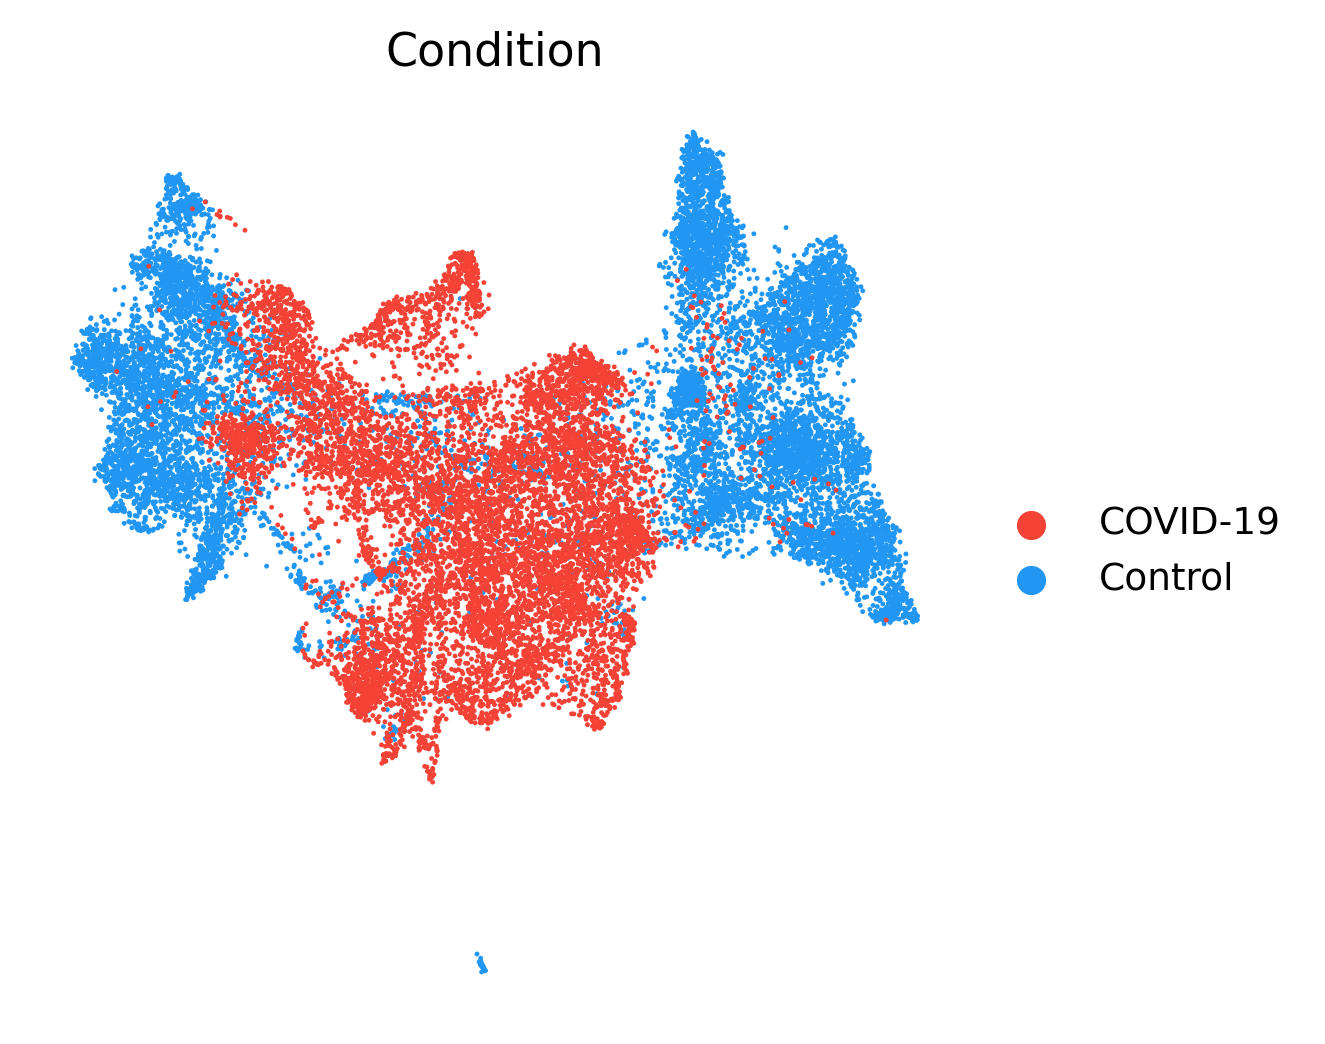
\includegraphics[width=0.62\linewidth]{fig1a_condition.png}
\caption{UMAP of all 22{,}128 alveolar cells. Each point is a cell. Colour =
Control (healthy) vs COVID-19.}
\end{figure}

\begin{resultbox}
\textbf{How to read it.} If Control and COVID cells cleanly split into
different regions, you'd see solid-colour blobs. They \emph{overlap},
meaning no mono-directional ``damage'' displacement. The COVID cloud is
more spread out --- the robustness-collapse pattern.
\end{resultbox}

\subsection{Figure 1b --- UMAP coloured by cell type}

\begin{figure}[H]\centering
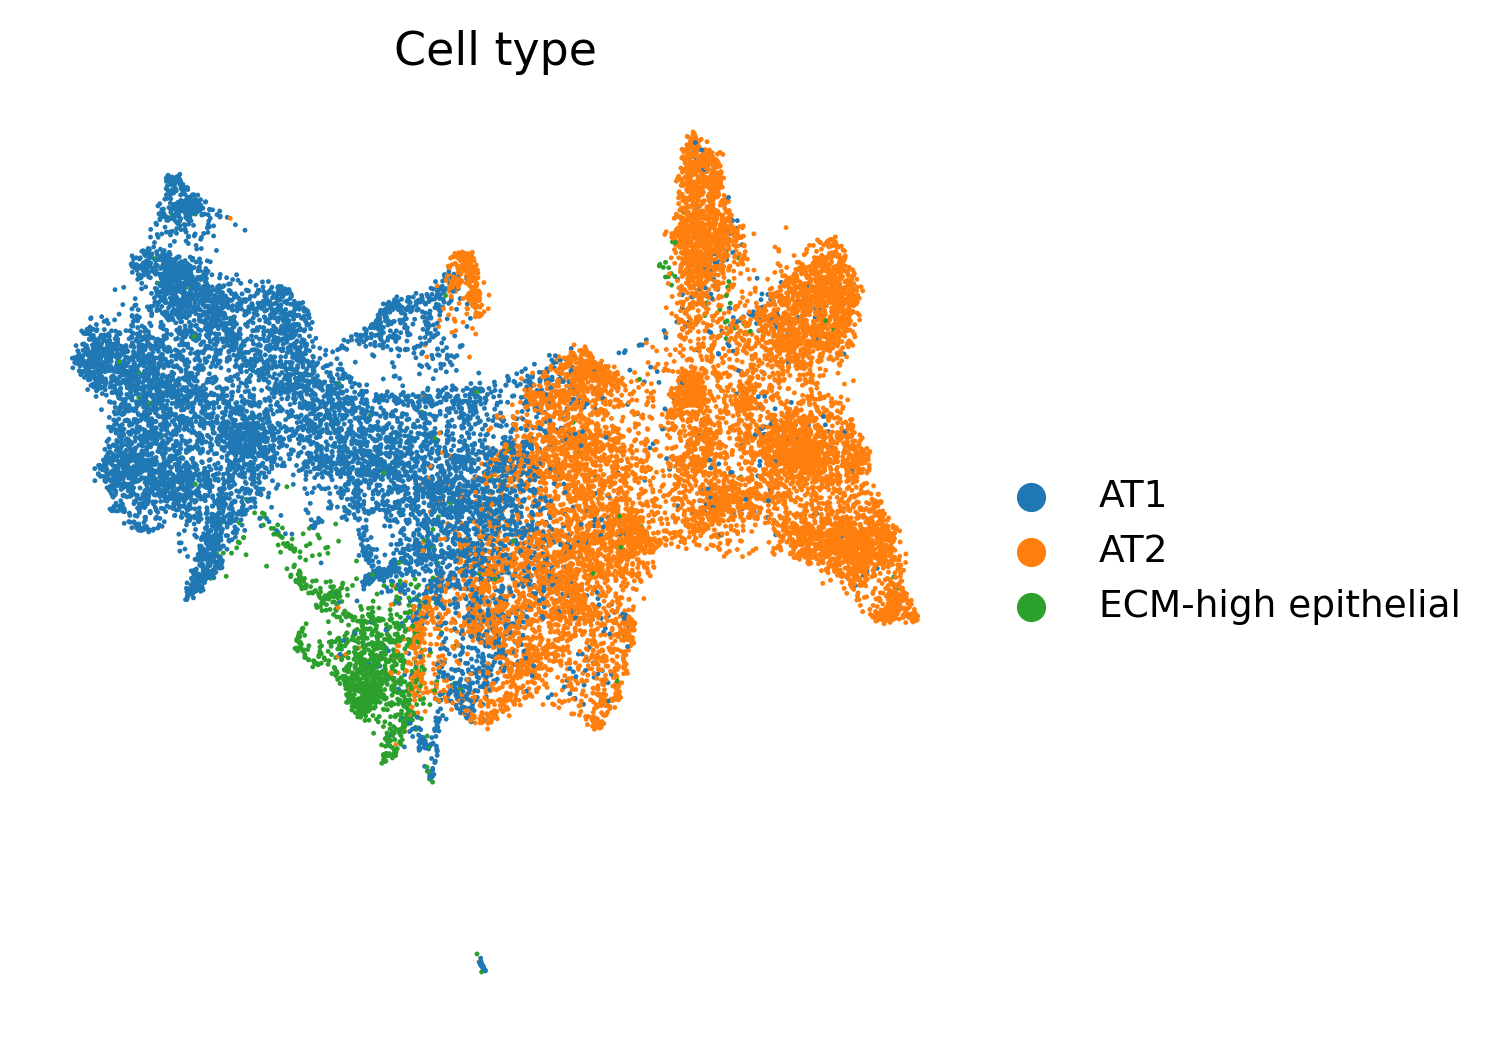
\includegraphics[width=0.62\linewidth]{fig1b_celltype.png}
\caption{Same UMAP, coloured by AT1 / AT2 / ECM-high.}
\end{figure}

\begin{resultbox}
Tells you the map has the right structure: AT2 dominates one region, AT1 the
other, and transitional cells sit between them. If cell types were
randomly scrambled on this map, we would not trust pseudotime on it.
\end{resultbox}

\subsection{Figure 2 --- UMAP coloured by pseudotime}

\begin{figure}[H]\centering
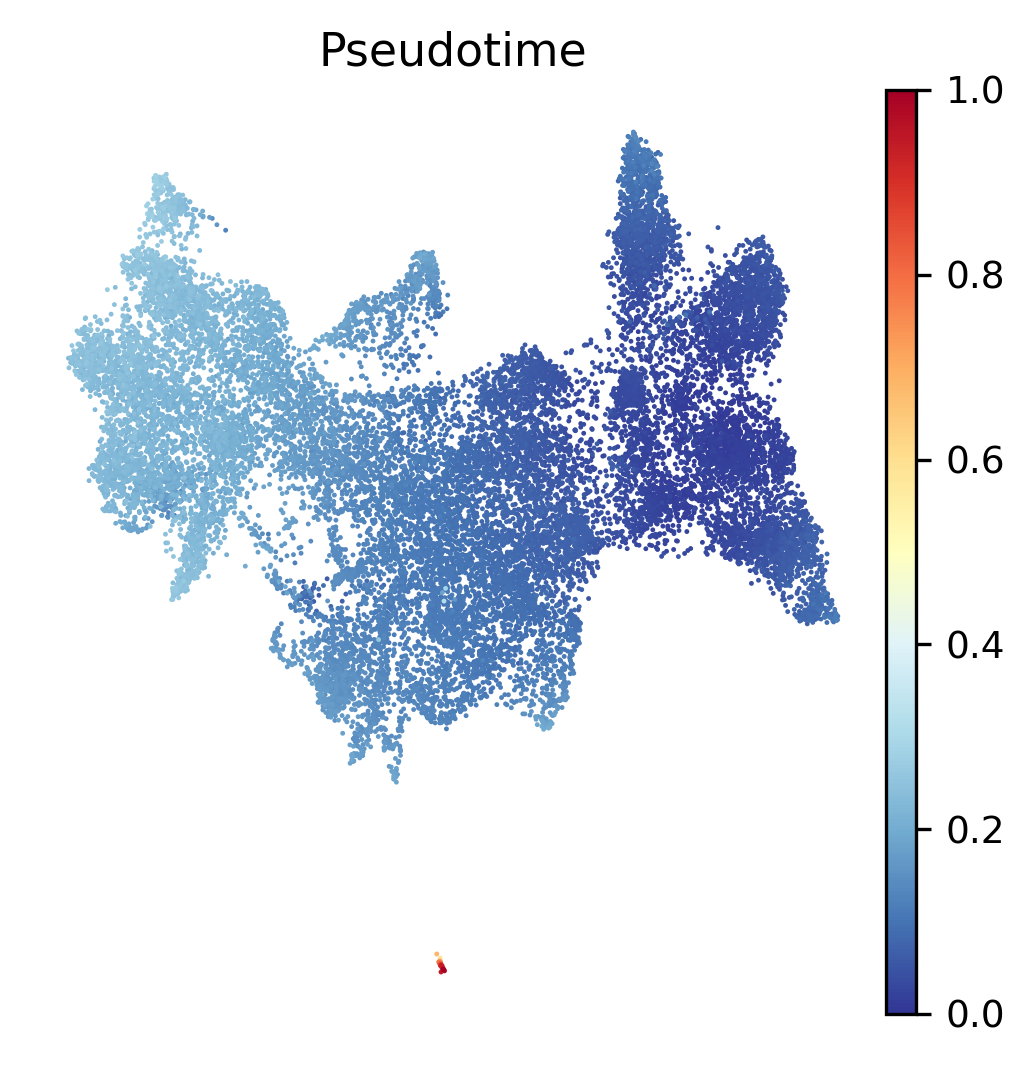
\includegraphics[width=0.62\linewidth]{fig2_pseudotime.png}
\caption{Every cell's pseudotime value on the UMAP.}
\end{figure}

\begin{resultbox}
Pseudotime (dark at root, light at furthest-forward) should grade smoothly
across the manifold. It does here: starting from healthy AT2, pseudotime
increases through the transitional region and out to the AT1 side. That's
the AT2$\to$DATP$\to$AT1 axis, ordered geometrically.
\end{resultbox}

\subsection{Figure 3 --- Program dynamics along pseudotime}

\begin{figure}[H]\centering
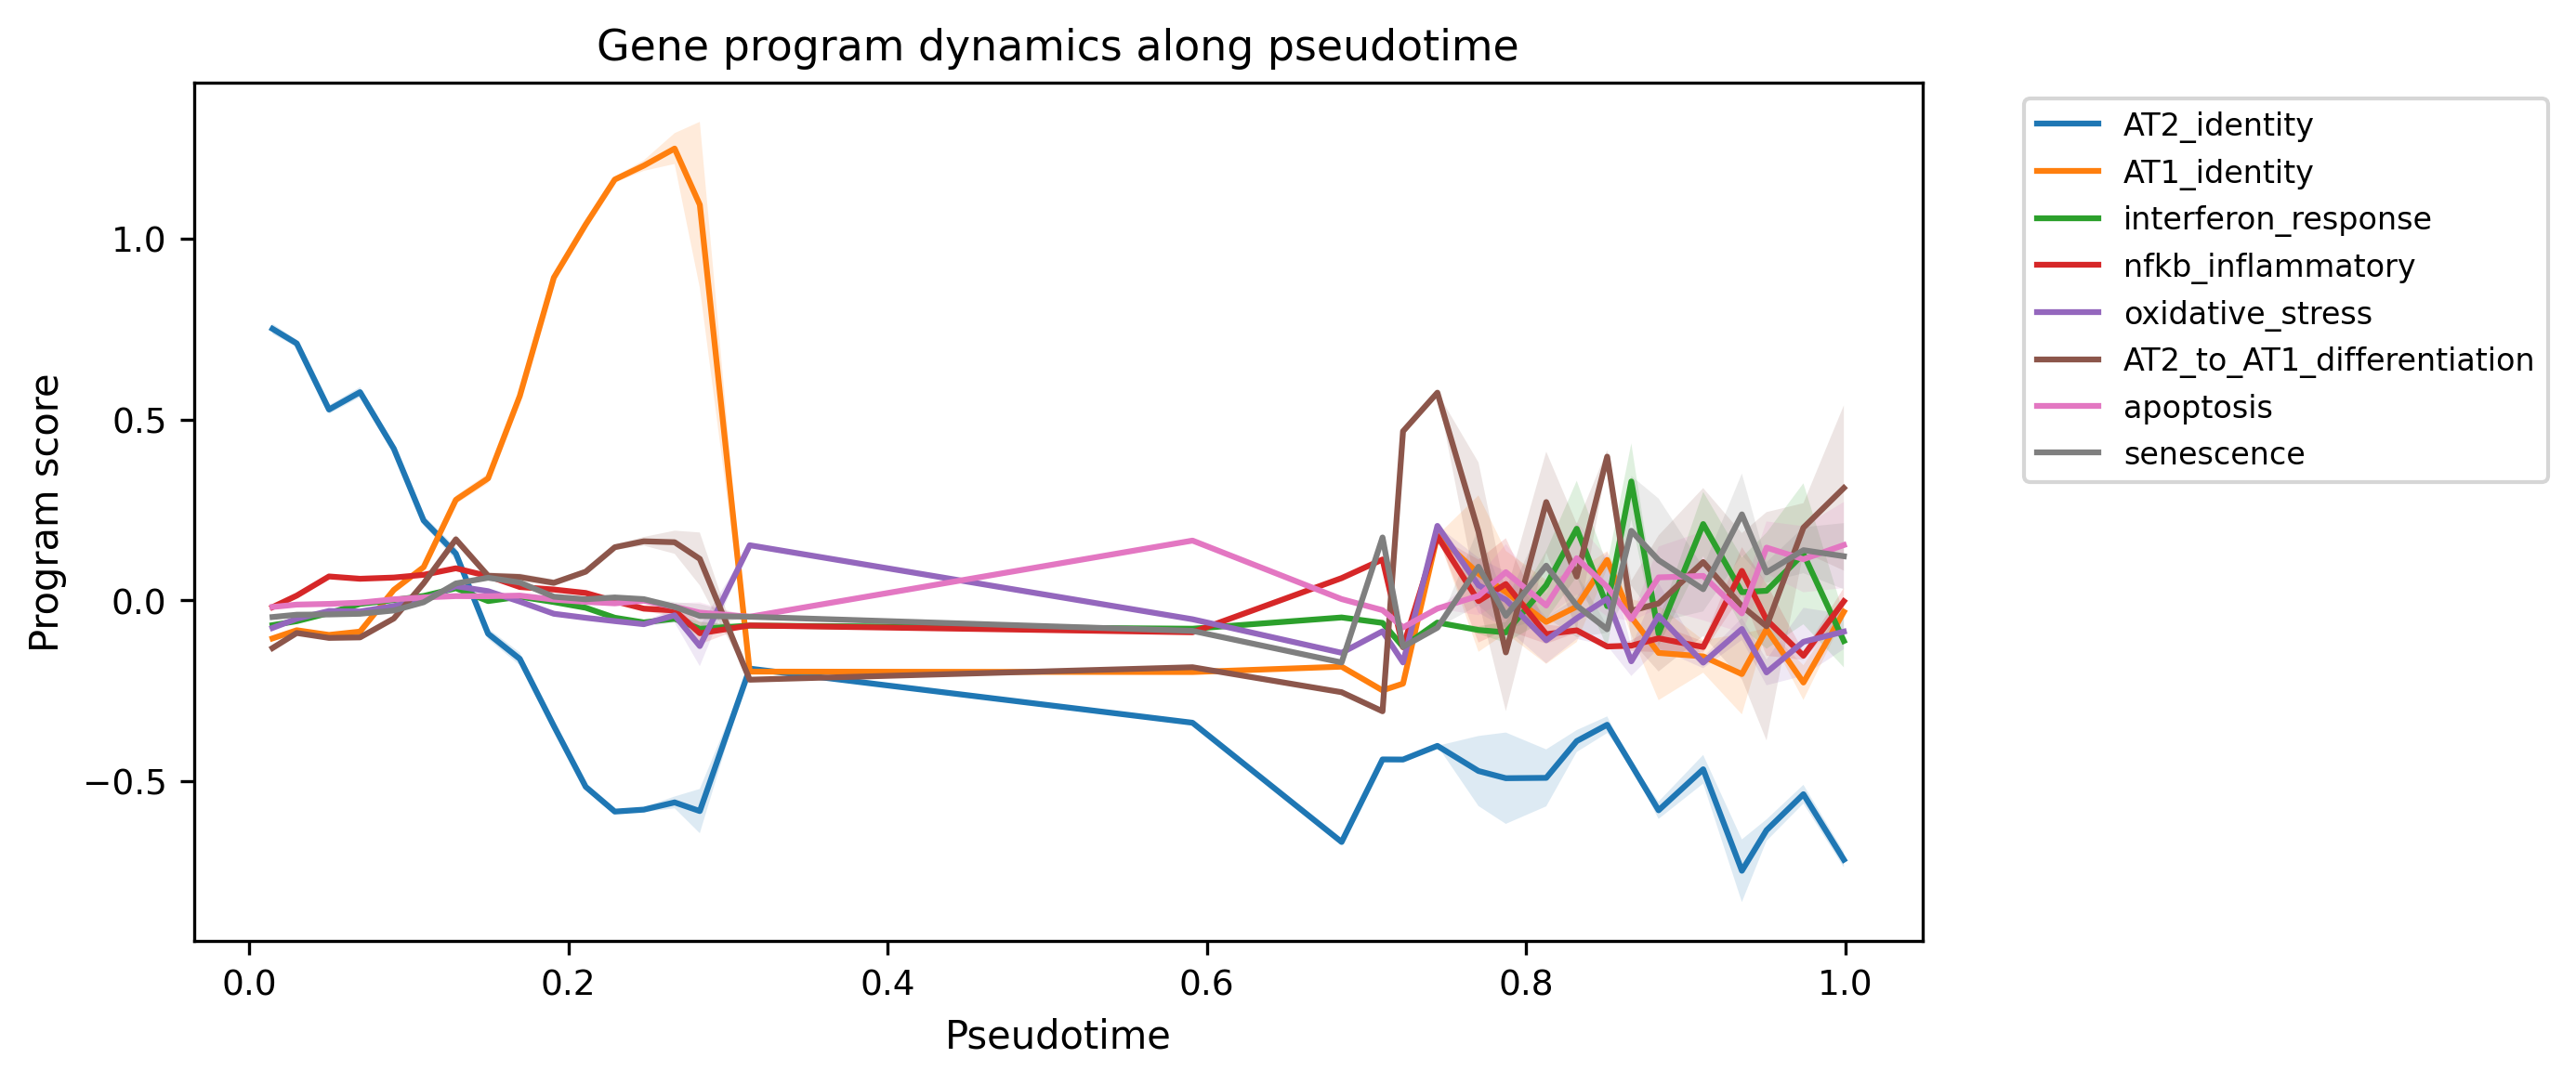
\includegraphics[width=0.85\linewidth]{fig3_program_dynamics.png}
\caption{Each panel: one gene program's score (y) plotted against
pseudotime (x), smoothed across cells.}
\end{figure}

\begin{resultbox}
Homeostatic programs (AT2 identity) decrease with pseudotime; injury-linked
programs (IFN, oxidative stress, AT2$\to$AT1) increase. This is the
expected biology and is used only as a sanity-check that the manifold
is capturing injury-state variation, \textbf{not} as an independent
statistical claim. (Ablation 8 is why I don't claim more: fine ordering
inverts under MSigDB.)
\end{resultbox}

\subsection{Figure 4 --- Pseudotime density by condition}

\begin{figure}[H]\centering
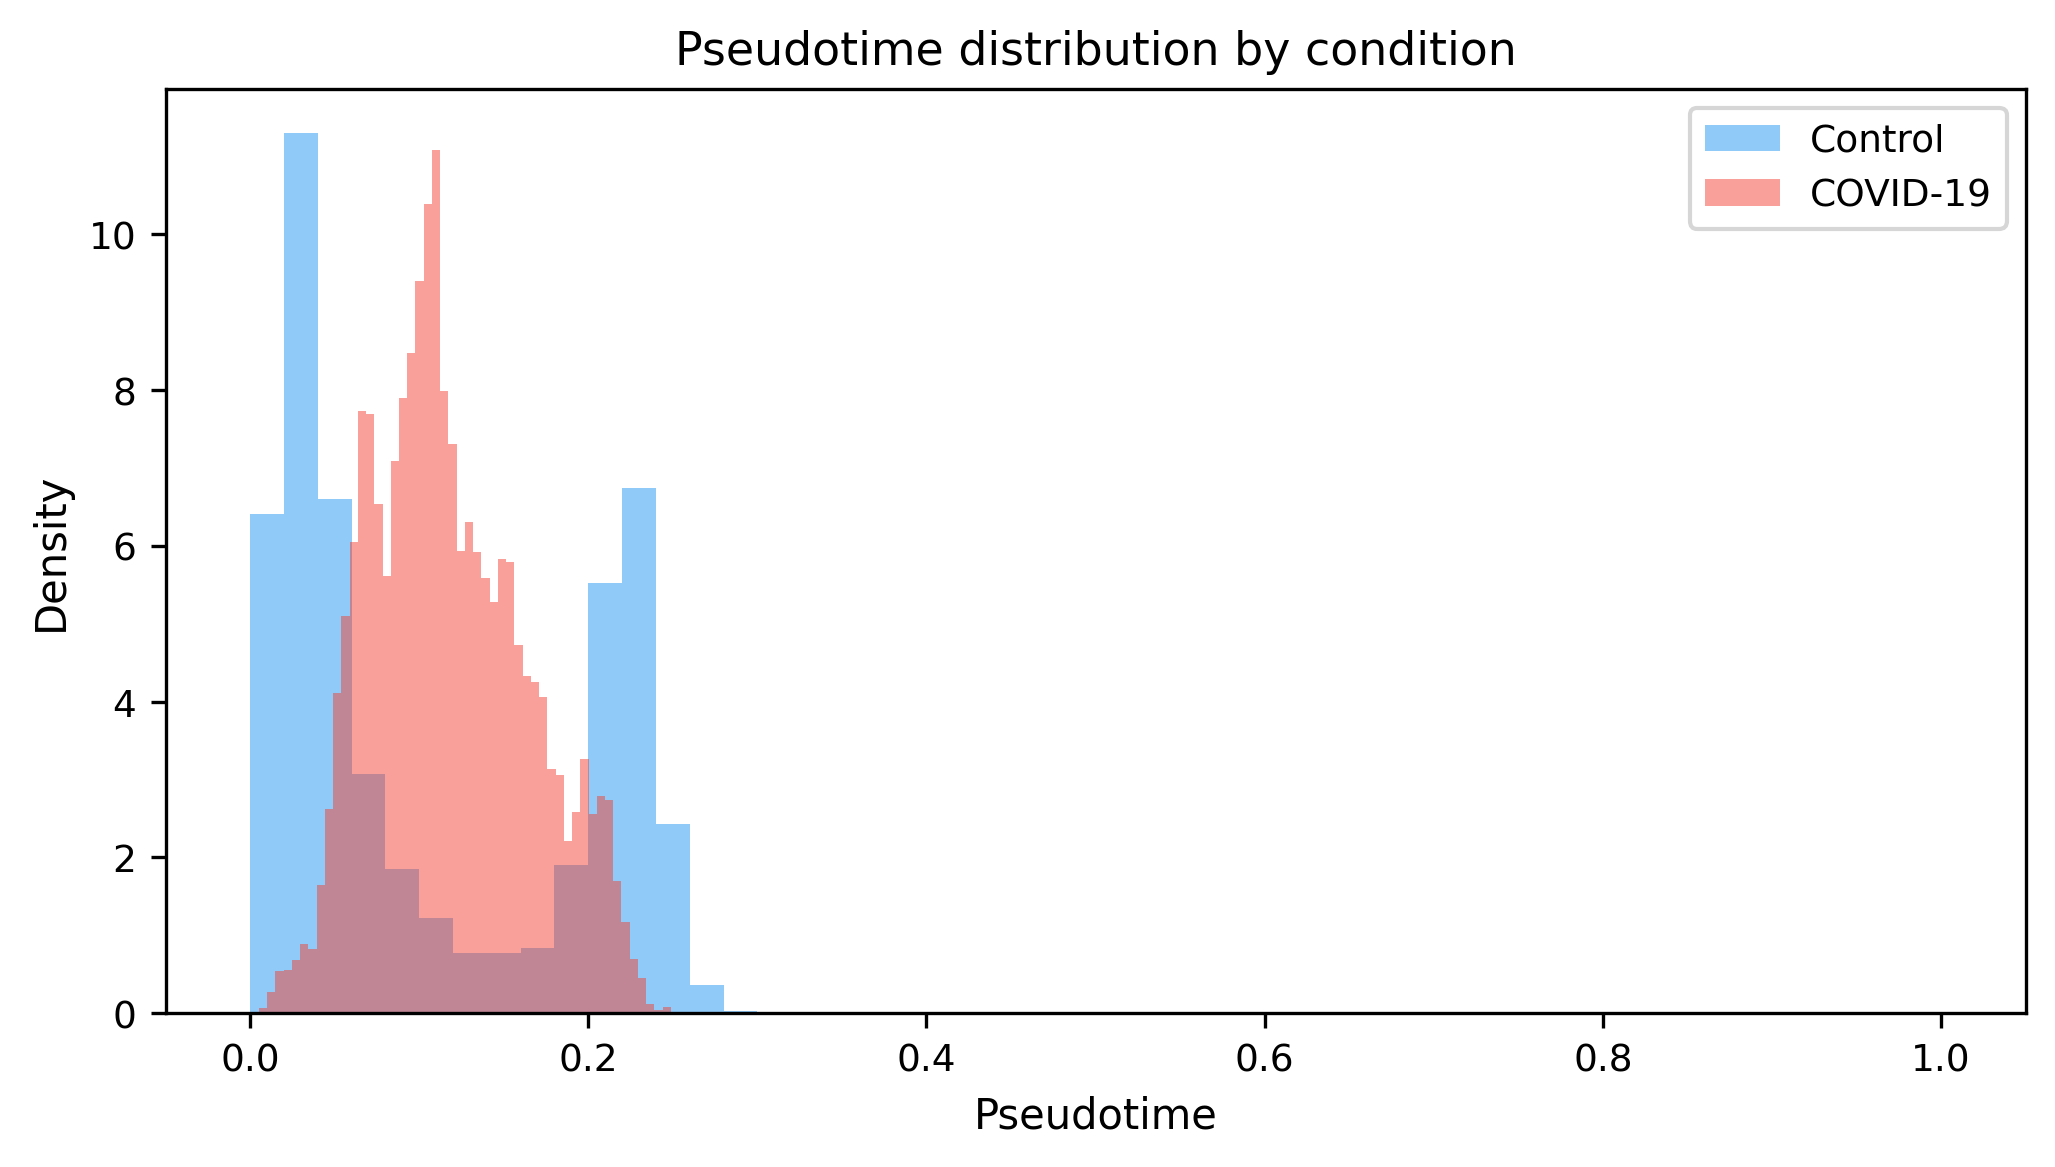
\includegraphics[width=0.55\linewidth]{fig4_pseudotime_density.png}
\caption{Kernel density estimates of pseudotime values. One curve per
condition.}
\end{figure}

\begin{resultbox}
\textbf{This is the core evidence for the pseudotime shift.}
Healthy curve is piled near the root; COVID curve has a fatter tail
toward higher pseudotime. Medians differ by $+0.0483$. Permutation
$p = 0.001$. LOO preserves direction in 27/27 donors.
\end{resultbox}

\subsection{Figure 5 --- Marker trends}

\begin{figure}[H]\centering
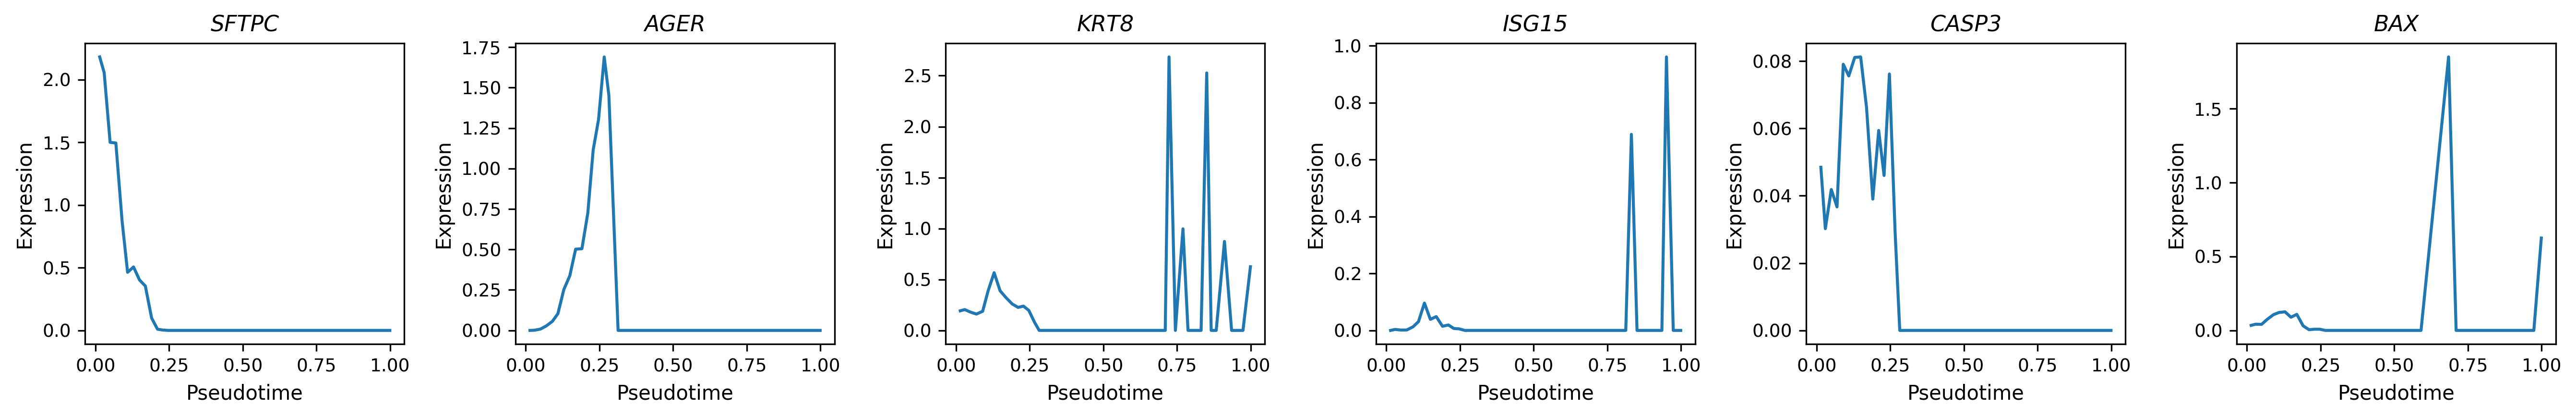
\includegraphics[width=0.8\linewidth]{fig5_marker_trends.png}
\caption{Per-marker smoothed expression along pseudotime.}
\end{figure}

\begin{resultbox}
AT2 markers (SFTPC) decrease along pseudotime; AT1 marker (AGER) increases;
transitional marker (KRT8) peaks in the middle; apoptosis marker (BAX) and
IFN marker (ISG15) increase. These are continuous-valued sanity checks that
the pseudotime ordering agrees with marker biology.
\end{resultbox}

\subsection{Figure 5b --- Displacement boxplot}

\begin{figure}[H]\centering
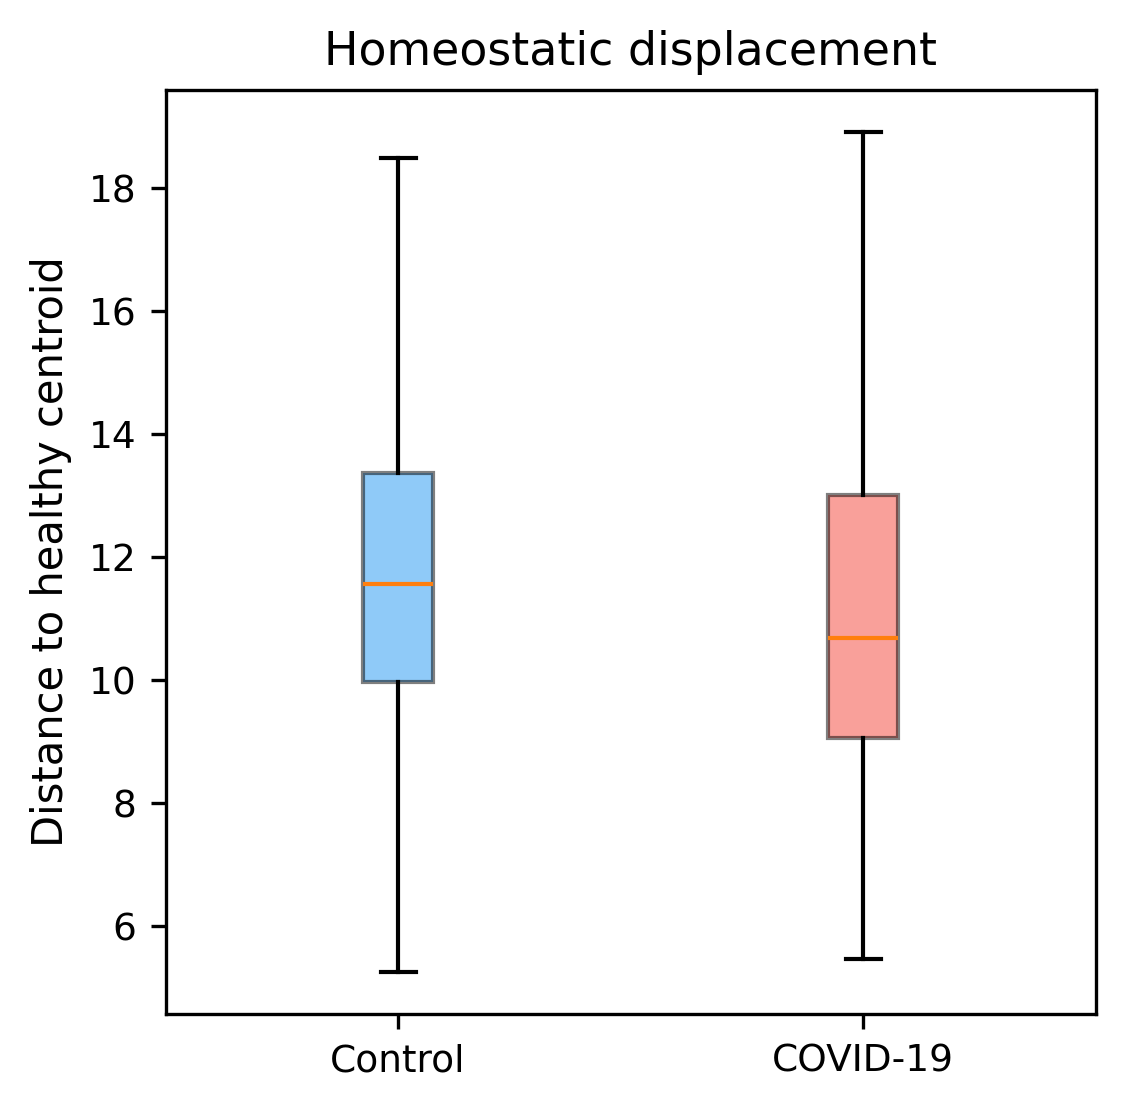
\includegraphics[width=0.55\linewidth]{fig5b_displacement.png}
\caption{Boxplot of per-cell distance to healthy centroid in PCA-50, by
condition.}
\end{figure}

\begin{resultbox}
\textbf{This is where the ``centroid displacement'' test fails.}
If the coordinated hypothesis were right, the COVID box should sit clearly
above the Healthy box. It does not. One-sided MW $p=1.0$; rank-biserial
$r=0.14$ \emph{in the wrong direction}. This is the most informative
failing test in the paper --- it rules out the
``monodirectional-damage-vector'' effect model.
\end{resultbox}

\subsection{Figure 7 --- Donor consistency}

\begin{figure}[H]\centering
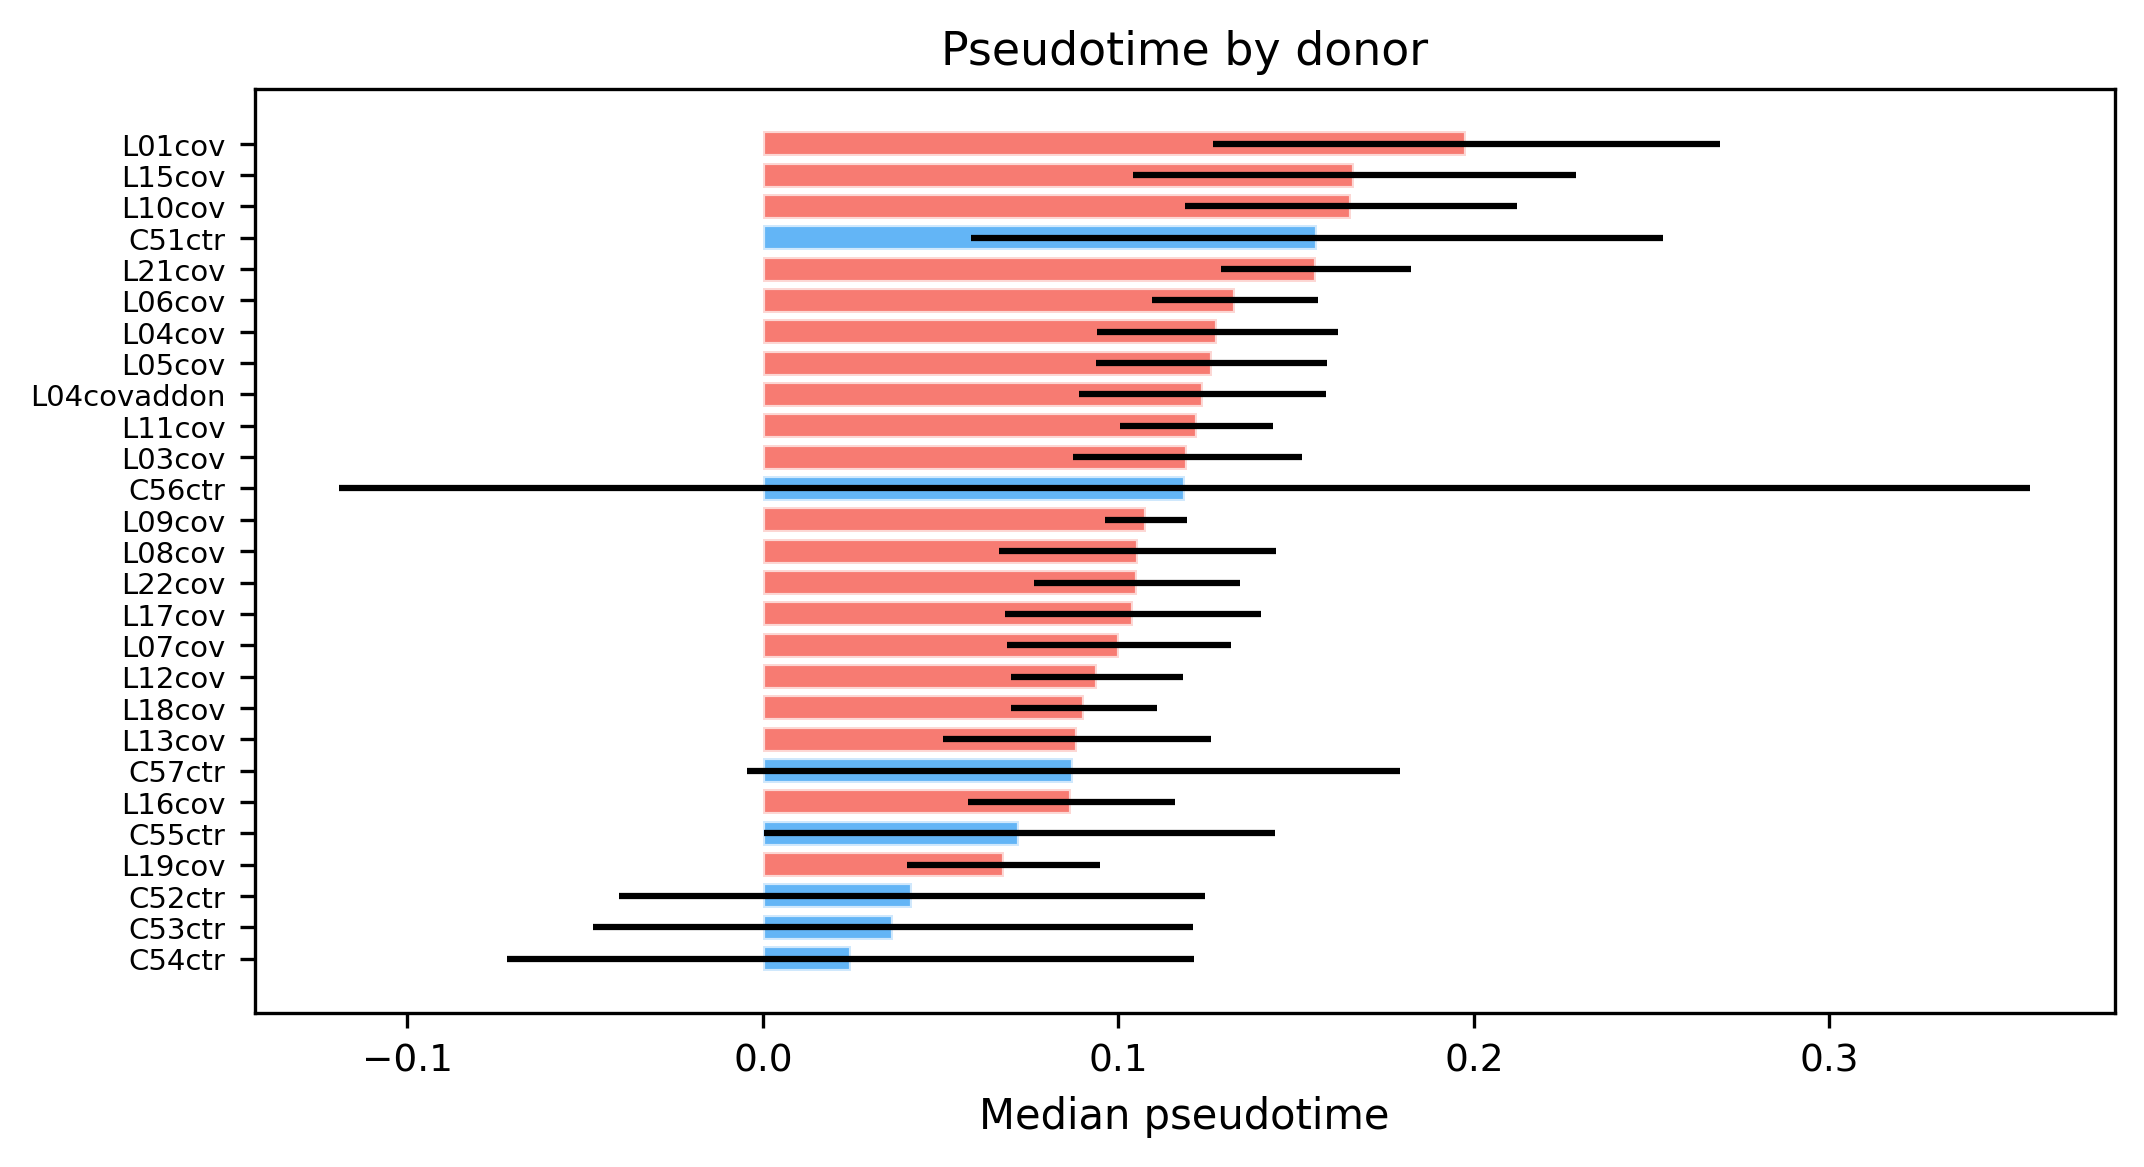
\includegraphics[width=0.68\linewidth]{fig7_donor_consistency.png}
\caption{Per-donor pseudotime summaries. Horizontal line = donor-level
median pseudotime; colour by condition.}
\end{figure}

\begin{resultbox}
Donors are ordered so you can see that COVID donors skew higher than healthy
donors individually, not because of 1--2 extreme donors. This, plus the
LOO 27/27 result, is what makes the pseudotime shift credible despite
the modest magnitude.
\end{resultbox}

% =========================================================================
\section{Part 8 --- Reading the tables}
% =========================================================================

\subsection{Table 2 --- robustness metrics}

[results/tables/table2\_robustness\_metrics.csv](results/tables/table2_robustness_metrics.csv)

Columns: each pre-registered test's test statistic, $p$-value, effect size,
and outcome (``supported'' / ``fails''). One row per test.

\subsection{Table 3 --- composite evidence}

[results/tables/table3\_composite\_evidence.csv](results/tables/table3_composite_evidence.csv)

A single row summarizing 2/3 of the pre-registered criteria supported,
1/3 failed. Used to argue that partial-pass with the \emph{right} failing
test is more informative than a uniform-pass.

\subsection{Table S6 --- ablations}

[results/ablations/tableS6\_ablation\_summary.csv](results/ablations/tableS6_ablation_summary.csv)

One row per ablation variant. Columns: MPD (median pseudotime difference),
$\rho$ (Spearman ordering of programs along pseudotime), $r$ (rank-biserial
displacement effect), notes. This is the table you stare at to see where the
analysis is brittle.

\subsection{Replication metrics JSON}

[results/replication/replication\_metrics.json](results/replication/replication_metrics.json)

Key numbers already reported above.

% =========================================================================
\section{Part 9 --- How the conclusion was assembled}
% =========================================================================

The conclusion is \textbf{not} ``we found a new COVID effect.'' The conclusion
is:

\begin{quote}
\emph{Of three pre-registered geometric tests for coordinated-block
versus robustness-collapse epithelial failure, the two that support
robustness collapse (dispersion, pseudotime shift) survive both a
10-axis ablation battery and an out-of-cohort replication in 618
independent donors; the one that would have supported
coordinated-block failure (centroid displacement) does not, in either
cohort. Therefore the best-supported model is robustness collapse,
and the mono-directional-damage model is ruled out.}
\end{quote}

The reason this is a valid conclusion from partial results is that the three
tests were designed ahead of time with opposing mechanistic meanings.
Having 2/3 succeed and 1/3 fail in a specific pattern is much more
informative than 3/3 succeeding: the failing test rules out a specific
alternative.

A secondary and equally important conclusion is methodological:

\begin{enumerate}
\item Batch correction \emph{matters}; Ablation 3 with the fixed Harmony
      shows that ``batch correction didn't help'' can mean ``my wrapper
      was broken'' rather than ``the method doesn't help''.
\item Marker-threshold cell-state classifiers like ``KRT8$^+$/CLDN4$^+$
      $\Rightarrow$ DATP'' do not transfer across cohorts. Manifold-based
      identification is needed.
\item Donor-level pseudobulk is the right unit of analysis for
      class-imbalanced cross-study replication.
\end{enumerate}

% =========================================================================
\section{Part 10 --- How to reproduce everything, end to end}
% =========================================================================

\subsection{Set up the environment}

\begin{verbatim}
cd /deltos/e/lesion_phes/code/python/pipeline/sb_class_project
python -m venv env
source env/bin/activate
pip install -r requirements.txt
\end{verbatim}

\subsection{Get the primary data}

\begin{verbatim}
python scripts/download_data.py        # fetches SCP1219 into data/raw/
\end{verbatim}

\subsection{Run the primary pipeline end-to-end}

\begin{verbatim}
python scripts/run_pipeline.py --step all
\end{verbatim}

Or step by step (handy for debugging):
\begin{verbatim}
python scripts/run_pipeline.py --step load_and_inspect
python scripts/run_pipeline.py --step qc
python scripts/run_pipeline.py --step subset
python scripts/run_pipeline.py --step embed
python scripts/run_pipeline.py --step trajectory
python scripts/run_pipeline.py --step programs
python scripts/run_pipeline.py --step stats
python scripts/run_pipeline.py --step figures
\end{verbatim}

Each step writes its outputs under \texttt{data/processed/}, \texttt{results/figures/},
or \texttt{results/tables/}. The \texttt{--skip-if-exists} flag lets you
restart without redoing finished steps.

\subsection{Run all ten ablations}

\begin{verbatim}
bash scripts/ablations/rerun_all.sh
\end{verbatim}

Each ablation writes its own sub-folder under \texttt{results/ablations/NN\_name/},
and \texttt{scripts/ablations/run\_all\_ablations.py} aggregates
the per-ablation metrics into
\texttt{results/ablations/tableS6\_ablation\_summary.csv}.

\subsection{Run the independent replication}

\begin{verbatim}
python scripts/replication/fetch_replication.py      # 89,736 cells download
python scripts/replication/analyze_replication.py    # statistics + JSON output
\end{verbatim}

Results land in \texttt{results/replication/replication\_metrics.json}.

% =========================================================================
\section{Part 11 --- Limitations I am honest about}
% =========================================================================

\begin{enumerate}
\item \textbf{Cross-sectional, post-mortem, lethal cases only} in the primary
      cohort. Nothing in this analysis tells you about moderate COVID.
\item \textbf{Replication gene panel too narrow} (84 genes) to build a new
      manifold. Full-transcriptome replication of the DPT itself is still
      missing.
\item \textbf{Replication does not include Delorey or Wendisch} (not on
      cellxgene census); would require raw GEO ingestion, which I did not do.
\item \textbf{Fine program ordering is hypothesis-generating only} ---
      Ablation 8 shows it inverts under alternative program definitions.
\item \textbf{Marker-threshold DATP enrichment retracted} as a portable
      statistic.
\item \textbf{Pseudotime is ordering, not elapsed time}; no claim about
      actual hours or stages.
\end{enumerate}

% =========================================================================
\section{Part 12 --- What to tell a friend in one sentence each}
% =========================================================================

\textbf{To a biologist:} In lethal COVID-19, alveolar epithelial cells don't
all move to one damaged state; they fan out along a graded axis, and this
``robustness collapse'' signature replicates in an independent 618-donor
atlas even though a marker-threshold DATP assay does not.

\textbf{To a computer scientist:} I pre-registered three geometric tests with
mutually exclusive mechanistic interpretations, ran ten ablations, fixed a
1-line Harmony orientation bug that changed the effect size 2.6$\times$, and
replicated in a held-out 35-dataset atlas at donor-level pseudobulk. The
methodological takeaway is that a failing pre-registered test is informative,
dispersion beats centroid displacement, and marker-threshold classifiers
don't transfer.

\textbf{To yourself:} The lung epithelium in lethal COVID doesn't collapse by
going somewhere new --- it collapses by spreading out, and the cleanest way
to see that is variance, not distance.

\end{document}
